\section{COS Trigonometric Cosine Function}

\subsection{Usage}

Computes the \verb|cos| function for its argument.  The general
syntax for its use is
\begin{verbatim}
  y = cos(x)
\end{verbatim}
where \verb|x| is an \verb|n|-dimensional array of numerical type.
Integer types are promoted to the \verb|double| type prior to
calculation of the \verb|cos| function.  Output \verb|y| is of the
same size and type as the input \verb|x|, (unless \verb|x| is an
integer, in which case \verb|y| is a \verb|double| type).  
\subsection{Function Internals}

Mathematically, the \verb|cos| function is defined for all real
valued arguments \verb|x| by the infinite summation
\[
  \cos x \equiv \sum_{n=0}^{\infty} \frac{(-1)^n x^{2n}}{(2n)!}.
\]
For complex valued arguments \verb|z|, the cosine is computed via
\[
  \cos z \equiv \cos \Re z \cosh \Im z - \sin \Re z
  \sinh \Im z.
\]
\subsection{Example}

The following piece of code plots the real-valued \verb|cos(2 pi x)|
function over one period of \verb|[0,1]|:
\begin{verbatim}
--> x = linspace(0,1);
--> plot(x,cos(2*pi*x))
\end{verbatim}


\centerline{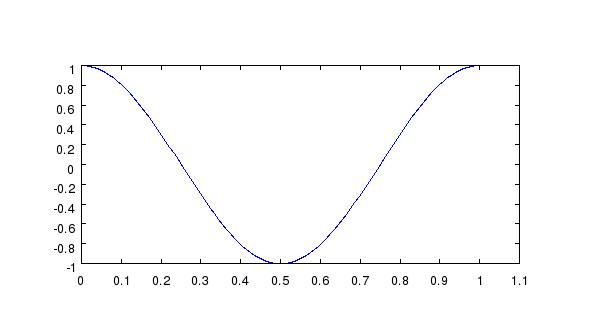
\includegraphics[width=8cm]{cosplot}}

